\chapter{Trasformata di Laplace e Diagrammi di Bode}
\label{ch:laplace-bode}

In questo capitolo viene introdotta la \textbf{trasformata di Laplace}, uno strumento matematico fondamentale per l'analisi dei circuiti lineari nel dominio della frequenza complessa. Successivamente, viene mostrato come costruire i \textbf{diagrammi di Bode}, che permettono di visualizzare in modo intuitivo il comportamento in frequenza di un circuito o di un sistema.

\section{La Trasformata di Laplace}

\subsection{Definizione e semipiano di convergenza}

La trasformata di Laplace è un'operazione integrale che mappa una funzione del tempo $f(t)$ (definita per $t \geq 0$) in una funzione $\tilde{f}(s)$ della variabile complessa $s \in \mathbb{C}$:

\begin{important}
\[
    \tilde{f}(s) = \mathcal{L}\{f(t)\} = \int_0^{+\infty} e^{-st} f(t) \, dt
\]
\end{important}

Il nucleo dell'integrale è $k(s,t) = e^{-st}$, con $s = \sigma + j\omega$ variabile complessa. Questa trasformata è la più generale di una famiglia di trasformate integrali: la \textbf{trasformata di Fourier} ne è un caso particolare, ottenuta restringendo la valutazione sull'asse immaginario, ovvero ponendo $s = j\omega$ con $\omega \in \mathbb{R}$.

La funzione $f(t)$ è assunta \textit{causale}, cioè $f(t) = 0$ per $t < 0$, il che giustifica il limite inferiore $0$ nell'integrale.

\vspace{0.5em}
\noindent\textbf{Convergenza dell'integrale.} L'integrale di Laplace non converge per ogni $s \in \mathbb{C}$. Supponiamo che $\exists\, s_0 = \sigma_0 + j\omega_0$ tale che $\tilde{f}(s_0)$ esista finita. Allora:
\[
    |\tilde{f}(s_0)| \leq \int_0^{+\infty} e^{-\sigma_0 t} |f(t)| \, dt < +\infty
\]

Per ogni $s$ con $\text{Re}(s) = \sigma \geq \sigma_0$, si ha $e^{-\sigma t} \leq e^{-\sigma_0 t}$, dunque:
\[
    |\tilde{f}(s)| \leq \int_0^{+\infty} e^{-\sigma t} |f(t)| \, dt \leq \int_0^{+\infty} e^{-\sigma_0 t} |f(t)| \, dt < +\infty
\]

Esiste quindi un valore $\overline{\sigma}$ (detto \textbf{ascissa di convergenza}) tale che l'integrale converge per ogni $s$ con $\text{Re}(s) > \overline{\sigma}$, e diverge per $\text{Re}(s) < \overline{\sigma}$. Il luogo dei punti in cui la trasformata è definita si chiama \textbf{semipiano di convergenza}.

\begin{figure}[H]
    \centering
    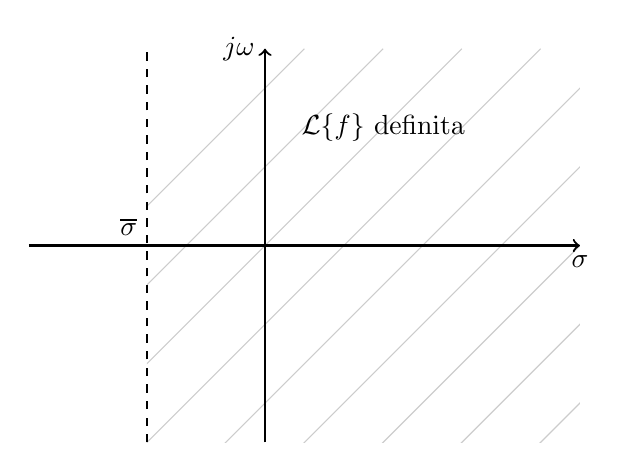
\begin{tikzpicture}
        \begin{scope}
            \clip (-1.5, -2.5) rectangle (4, 2.5);
            \foreach \x in {-5, -4, ..., 4} {
                \draw[gray!40] (\x, -3) -- (\x+5.5, 2.5);
            }
        \end{scope}
        \draw[->, thick] (-3,0) -- (4,0) node[below] {$\sigma$};
        \draw[->, thick] (0,-2.5) -- (0,2.5) node[left] {$j\omega$};
        \draw[dashed, thick] (-1.5, -2.5) -- (-1.5, 2.5);
        \node[above left] at (-1.5, 0) {$\overline{\sigma}$};
        \node at (1.5, 1.5) {$\mathcal{L}\{f\}$ definita};
    \end{tikzpicture}
    \caption{Semipiano di convergenza: la trasformata di Laplace è definita nella regione tratteggiata, ovvero per $\text{Re}(s) > \overline{\sigma}$.}
\end{figure}

\vspace{0.3em}
\noindent\textbf{Esempi di ascissa di convergenza:}
\begin{itemize}
    \item $f(t) = a_n t^n + \dots + a_0$ (polinomio) $\;\Rightarrow\; \overline{\sigma} = 0$
    \item $f(t) = e^{at}$ $\;\Rightarrow\; \overline{\sigma} = a$
    \item $f(t) = e^{-bt^2}$ con $b > 0$ $\;\Rightarrow\; \overline{\sigma} = -\infty$ (la trasformata esiste su tutto $\mathbb{C}$)
    \item $f(t) = e^{ct^2}$ con $c > 0$ $\;\Rightarrow\; \overline{\sigma} = +\infty$ (la trasformata non esiste in alcun punto)
\end{itemize}

\subsection{Proprietà fondamentali}

\subsubsection*{Linearità}
La trasformata di Laplace è un operatore lineare: dati $a_1, a_2 \in \mathbb{C}$ e due funzioni $f_1(t), f_2(t)$,
\[
    \mathcal{L}\{a_1 f_1(t) + a_2 f_2(t)\} = a_1 \mathcal{L}\{f_1(t)\} + a_2 \mathcal{L}\{f_2(t)\}
\]

\subsubsection*{Analiticità}
Nel semipiano di convergenza, $\tilde{f}(s)$ è una funzione analitica (olomorfa) di $s$. Ciò si verifica derivando sotto il segno di integrale:
\[
    \frac{d\tilde{f}}{ds} = \frac{d}{ds} \int_0^{+\infty} e^{-st} f(t) \, dt = -\int_0^{+\infty} t \, f(t) \, e^{-st} \, dt = -\mathcal{L}\{t\, f(t)\}
\]
Iterando:
\[
    \frac{d^n \tilde{f}}{ds^n} = (-1)^n \mathcal{L}\{t^n f(t)\}
\]
Poiché tutte le derivate esistono, $\tilde{f}(s)$ è analitica. Le eventuali singolarità si trovano dunque a sinistra del semipiano di convergenza (o al più sulla sua frontiera).

\subsubsection*{Traslazione in frequenza}
Se $f(t) \xrightarrow{\mathcal{L}} \tilde{f}(s)$, allora per ogni $a \in \mathbb{C}$:
\[
    \mathcal{L}\{e^{at} f(t)\} = \tilde{f}(s - a)
\]
L'ascissa di convergenza di $e^{at} f(t)$ vale $\overline{\sigma} + \text{Re}(a)$.

\subsubsection*{Traslazione temporale}
Per $t_0 > 0$ e $f$ causale (quindi $f(t-t_0) = 0$ per $t < t_0$):
\[
    \mathcal{L}\{f(t - t_0)\} = \int_{t_0}^{+\infty} f(t - t_0) e^{-st} \, dt \overset{\tau = t - t_0}{=} \int_0^{+\infty} f(\tau) e^{-s(\tau + t_0)} \, d\tau = e^{-s t_0} \tilde{f}(s)
\]

\subsubsection*{Convoluzione}
Siano $f(t)$ e $g(t)$ due funzioni causali. Nel semipiano intersezione dei semipiani di convergenza di $f$ e $g$, la trasformata della loro convoluzione è il prodotto delle trasformate:
\[
    \mathcal{L}\{f * g\} = \tilde{f}(s) \cdot \tilde{g}(s)
\]

\subsubsection*{Derivazione nel tempo}
Per una funzione $f \in C^1(\mathbb{R}^+)$, integrando per parti:
\[
    \mathcal{L}\{f'(t)\} = s\tilde{f}(s) - f(0^+)
\]
La derivazione nel tempo corrisponde a una moltiplicazione per $s$ nel dominio di Laplace, convertendo equazioni differenziali in equazioni algebriche.

\subsubsection*{Integrazione nel tempo}
In modo duale, l'integrazione nel tempo corrisponde alla divisione per $s$:
\[
    \mathcal{L}\left\{\int_0^t f(t') \, dt'\right\} = \frac{\tilde{f}(s)}{s}
\]

\subsection{Trasformate notevoli}

\begin{table}[H]
    \centering
    \renewcommand{\arraystretch}{1.8}
    \begin{tabular}{lc}
        \toprule
        \textbf{Funzione del tempo} $f(t)$ & \textbf{Trasformata di Laplace} $\tilde{f}(s)$ \\
        \midrule
        $\delta(t)$ (impulso di Dirac) & $1$ \\
        $u(t) = 1$ (gradino unitario) & $\dfrac{1}{s}$ \\
        $t^n$ & $\dfrac{n!}{s^{n+1}}$ \\
        $e^{at}$ & $\dfrac{1}{s - a}$ \\
        $\cos(\omega t)$ & $\dfrac{s}{s^2 + \omega^2}$ \\
        $\sin(\omega t)$ & $\dfrac{\omega}{s^2 + \omega^2}$ \\
        $f'(t)$ & $s\tilde{f}(s) - f(0^+)$ \\
        \bottomrule
    \end{tabular}
    \caption{Principali coppie di trasformate di Laplace.}
\end{table}

\subsection{Applicazione: risoluzione di un circuito RC}

Consideriamo il seguente circuito RC: alla chiusura dell'interruttore, il condensatore si carica attraverso la resistenza $R$.

\begin{fitcenter}
\begin{circuitikz}[american, transform shape]
    \draw (0,0) to[battery1, l=$V_0$] (0,2)
    to[nos] (1,2)
    to[R=$R$] (3,2)
    to[C=$C$] (3,0) -- (0,0);
    \draw (3,2) -- (4,2);
    \draw (3,0) -- (4,0);
    \draw[<->] (4,0.2) -- (4,1.8) node[midway, right] {$V_{\text{out}}$};
    \draw (4,0) circle (2pt);
    \draw (4,2) circle (2pt);
\end{circuitikz}
\end{fitcenter}

Scrivendo la LKT sulla maglia con $\tau = RC$:
\[
    \dot{V}_{\text{out}} + \frac{1}{\tau} V_{\text{out}} = \frac{V_0}{\tau}, \qquad V_{\text{out}}(0^+) = \frac{Q(0)}{C}
\]
Applicando la trasformata di Laplace (e usando $\mathcal{L}\{\dot{V}_{\text{out}}\} = s\tilde{V}_{\text{out}} - V_{\text{out}}(0^+)$):
\[
    \left(s + \frac{1}{\tau}\right)\tilde{V}_{\text{out}} = \frac{V_0}{\tau s} + V_{\text{out}}(0^+)
    \quad\Longrightarrow\quad
    \tilde{V}_{\text{out}} = V_0\!\left[\frac{1}{s} - \frac{1}{s+\frac{1}{\tau}}\right] + \frac{V_{\text{out}}(0^+)}{s+\frac{1}{\tau}}
\]
Antitrasformando con la coppia $\mathcal{L}^{-1}\!\left\{\frac{1}{s-a}\right\} = e^{at}$:
\[
    V_{\text{out}}(t) = V_0\!\left(1 - e^{-t/\tau}\right) + V_{\text{out}}(0^+)\, e^{-t/\tau}
\]
Il primo termine è la \textit{risposta forzata} (carica verso $V_0$), il secondo è la \textit{risposta libera} (scarica delle condizioni iniziali), entrambe con costante di tempo $\tau = RC$.

\section{Impedenze Generalizzate e Funzione di Trasferimento}

\subsection{Impedenze nel dominio di Laplace}

Applicando la trasformata di Laplace (con condizioni iniziali nulle) alle leggi costitutive dei componenti si ottengono le \textbf{impedenze generalizzate}:
$Z_R = R$, $Z_C = \frac{1}{sC}$, $Z_L = sL$.

\subsection{Funzione di trasferimento}

La \textbf{funzione di trasferimento} $\tilde{A}(s) = \frac{\tilde{V}_{\text{out}}(s)}{\tilde{V}_{\text{in}}(s)}$ descrive il comportamento del sistema. È una funzione razionale i cui poli $p_k$ (zeri del denominatore) devono avere $\text{Re}(p_k) < 0$ per garantire la stabilità del sistema.

\begin{itemize}
    \item \textbf{Filtro passa-basso RC:} $\tilde{A}(s) = \frac{1}{1 + sRC}$ — polo del $1^\circ$ ordine in $s = -1/\tau$.
    \item \textbf{Filtro passa-alto RC:} $\tilde{A}(s) = \frac{sRC}{1 + sRC}$ — zero in $s=0$, polo in $s = -1/\tau$.
    \item \textbf{Circuito integratore} (Op-Amp con retroazione capacitiva):
\end{itemize}

\begin{fitcenter}
\begin{circuitikz}[american, transform shape]
    \draw (0,0) node[op amp] (opamp) {};
    \draw (opamp.-) to[R=$R_1$] (-3,0.5) node[left] {$V_S$};
    \draw (opamp.+) to[short] (-1.2,-0.5) node[ground] {};
    \draw (opamp.-) -- (-1.2,1.5) to[C=$C$] (1.2,1.5) -- (opamp.out);
    \draw (-1.2,1.5) -- (-1.2, 2.5) to[R=$R_2$] (1.2,2.5) -- (1.2,1.5);
    \draw (opamp.out) to[short, -o] (1.5,0) node[right] {$V_{\text{out}}$};
\end{circuitikz}
\end{fitcenter}

La funzione di trasferimento è $\tilde{A}(s) = -\frac{R_2}{R_1} \cdot \frac{1}{1 + s R_2 C}$. Nel limite $R_2 \to \infty$ si ottiene l'integratore ideale:
\[
    \tilde{A}(s) \xrightarrow{R_2 \to \infty} -\frac{1}{s R_1 C}
    \quad\Longrightarrow\quad
    V_{\text{out}}(t) = -\frac{1}{R_1 C} \int_{t_0}^t V_s(t') \, dt'
\]

\section{Diagrammi di Bode}

I \textbf{diagrammi di Bode} sono grafici in scala semilogaritmica che rappresentano il modulo e la fase della funzione di trasferimento $\tilde{A}(j\omega)$ in funzione della frequenza angolare $\omega$. Sono uno strumento essenziale per la progettazione e l'analisi dei circuiti in frequenza.

\subsection{Costruzione dei diagrammi asintotici}

Data la funzione di trasferimento in forma fattorizzata:
\[
    \tilde{A}(s) = K \frac{\prod_k (s - z_k)}{\prod_k (s - p_k)}
\]
valutata sull'asse immaginario ($s = j\omega$):
\[
    A(j\omega) = K \frac{\prod_k (j\omega - z_k)}{\prod_k (j\omega - p_k)}
\]

Il \textbf{diagramma di Bode in ampiezza} rappresenta:
\[
    A_{\text{dB}}(\omega) = 20\log_{10}|A(j\omega)| = 20\log_{10}|K| + \sum_k 20\log_{10}|j\omega - z_k| - \sum_k 20\log_{10}|j\omega - p_k|
\]

Il contributo di ogni fattore si analizza separatamente; i risultati si sommano grazie alla linearità del logaritmo.

\subsubsection*{Contributo di uno zero reale di ordine $m_k$ in $s = \sigma_k < 0$}

\[
    |j\omega - \sigma_k| = \sqrt{\omega^2 + \sigma_k^2}
\]

\begin{itemize}
    \item Per $\omega \ll |\sigma_k|$: $\quad |j\omega - \sigma_k|^{m_k} \approx |\sigma_k|^{m_k}$ \quad(costante)
    \item Per $\omega \gg |\sigma_k|$: $\quad |j\omega - \sigma_k|^{m_k} \approx \omega^{m_k}$ \quad($+20m_k$ dB/decade)
\end{itemize}

$\Rightarrow$ al passaggio della frequenza di rottura $\omega = |\sigma_k|$, la pendenza del diagramma di Bode \textbf{aumenta} di $+20\,m_k$ dB/decade (equivalente a $+6\,m_k$ dB/ottava).

\subsubsection*{Contributo di un polo reale di ordine $n_k$ in $s = p_k < 0$}

\[
    |j\omega - p_k|^{n_k} = \left(\sqrt{\omega^2 + p_k^2}\right)^{n_k}
\]

\begin{itemize}
    \item Per $\omega \ll |p_k|$: $\quad |j\omega - p_k|^{n_k} \approx |p_k|^{n_k}$ \quad(costante)
    \item Per $\omega \gg |p_k|$: $\quad |j\omega - p_k|^{n_k} \approx \omega^{n_k}$ \quad($-20n_k$ dB/decade)
\end{itemize}

$\Rightarrow$ al passaggio della frequenza di rottura $\omega = |p_k|$, la pendenza del diagramma di Bode \textbf{diminuisce} di $20\,n_k$ dB/decade (varia di $-20\,n_k$ dB/decade).

\subsubsection*{Contributo sulla fase}

Il \textbf{diagramma di Bode in fase} rappresenta:
\[
    \phi(\omega) = \arg A(j\omega) = \arg(K) + \sum_k \arg(j\omega - z_k) - \sum_k \arg(j\omega - p_k)
\]

\begin{itemize}
    \item \textbf{Zero reale negativo} $z_k < 0$: la fase varia da $0$ a $+\frac{\pi}{2}\,m_k$ attraversando $\omega = |z_k|$. Variazione totale: $+\frac{\pi}{2}\,m_k$.
    \item \textbf{Polo reale negativo} $p_k < 0$: la fase varia da $0$ a $-\frac{\pi}{2}\,n_k$ attraversando $\omega = |p_k|$. Variazione totale: $-\frac{\pi}{2}\,n_k$.
    \item \textbf{Zero reale positivo} $z_k > 0$ (sistema a fase non minima): la variazione di fase è $-\frac{\pi}{2}\,m_k$ (opposta a quella di uno zero negativo).
\end{itemize}

\subsection{Esempi di diagrammi di Bode}

\subsubsection*{Filtro passa-basso: $\tilde{A}(s) = \dfrac{1}{1+sRC}$}

Polo in $s = -\frac{1}{\tau}$ con $\tau = RC$. Per $\omega < \frac{1}{\tau}$ il modulo è circa $0$ dB; per $\omega > \frac{1}{\tau}$ il modulo cala di $-20$ dB/decade. Alla frequenza di taglio $\omega = \frac{1}{\tau}$ il modulo vale $-3$ dB e la fase vale $-45^\circ$.

\begin{fitcenter}
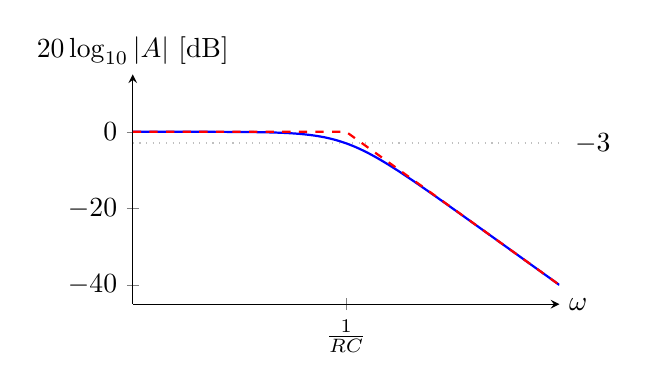
\begin{tikzpicture}
\begin{axis}[
    width=7cm, height=4.5cm,
    xmode=log,
    xlabel={$\omega$},
    ylabel={$20 \log_{10} |A|$ [dB]},
    axis lines=left,
    xmin=0.1, xmax=100,
    xmin=0.01, xmax=100,
    ymin=-45, ymax=15,
    xtick={1}, xticklabels={$\frac{1}{RC}$},
    ytick={0,-20,-40},
    extra y tick style={grid=major, grid style={dotted,thick}, yticklabel pos=right},
    extra y ticks={-3},
    domain=0.01:100, samples=200,
    every axis x label/.style={at={(ticklabel* cs:1)},anchor=west},
    every axis y label/.style={at={(ticklabel* cs:1)},anchor=south},
]
\addplot[blue, thick] {20*log10(1/sqrt(1+(x)^2))};
\addplot[red, dashed, thick] coordinates {(0.01,0) (1,0) (100,-40)};
\end{axis}
\end{tikzpicture}
%
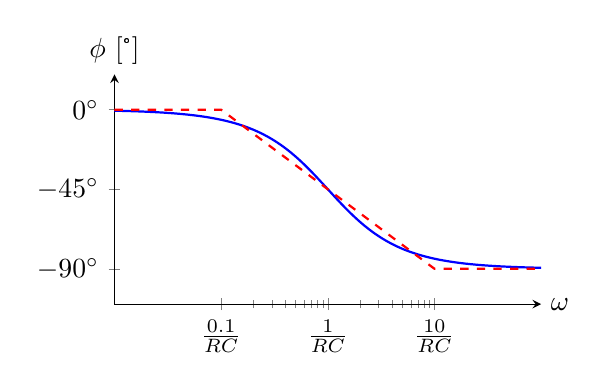
\begin{tikzpicture}
\begin{axis}[
    width=7cm, height=4.5cm,
    xmode=log,
    xlabel={$\omega$},
    ylabel={$\phi$ [°]},
    axis lines=left,
    xmin=0.1, xmax=100,
    xmin=0.01, xmax=100,
    ymin=-110, ymax=20,
    xtick={0.1, 1, 10}, xticklabels={$\frac{0.1}{RC}$, $\frac{1}{RC}$, $\frac{10}{RC}$},
    ytick={0, -45, -90}, yticklabels={$0^\circ$, $-45^\circ$, $-90^\circ$},
    domain=0.01:100, samples=200,
    every axis x label/.style={at={(ticklabel* cs:1)},anchor=west},
    every axis y label/.style={at={(ticklabel* cs:1)},anchor=south},
]
\addplot[blue, thick] {-atan(x)};
\addplot[red, dashed, thick] coordinates {(0.01,0) (0.1,0) (1,-45) (10,-90) (100,-90)};
\end{axis}
\end{tikzpicture}
\end{fitcenter}

\subsubsection*{Filtro passa-alto: $\tilde{A}(s) = \dfrac{sRC}{1+sRC}$}

Zero in $s = 0$, polo in $s = -\frac{1}{\tau}$. Per $\omega \ll \frac{1}{\tau}$ il modulo cresce con $+20$ dB/decade; per $\omega \gg \frac{1}{\tau}$ il modulo è circa $0$ dB.

\begin{fitcenter}
\begin{tikzpicture}
\begin{axis}[
    width=7cm, height=4.5cm,
    xmode=log,
    xlabel={$\omega$},
    ylabel={$|A|_{\text{dB}}$},
    axis lines=left,
    xmin=0.1, xmax=100,
    xmin=0.01, xmax=100,
    ymin=-45, ymax=15,
    xtick={1}, xticklabels={$\frac{1}{RC}$},
    ytick={0,-20,-40},
    extra y tick style={grid=major, grid style={dotted,thick}, yticklabel pos=right},
    extra y ticks={-3},
    domain=0.01:100, samples=200,
    every axis x label/.style={at={(ticklabel* cs:1)},anchor=west},
    every axis y label/.style={at={(ticklabel* cs:1)},anchor=south},
]
\addplot[blue, thick] {20*log10(x/sqrt(1+(x)^2))};
\addplot[red, dashed, thick] coordinates {(0.01,-40) (0.1,-20) (1,0) (100,0)};
\end{axis}
\end{tikzpicture}
%
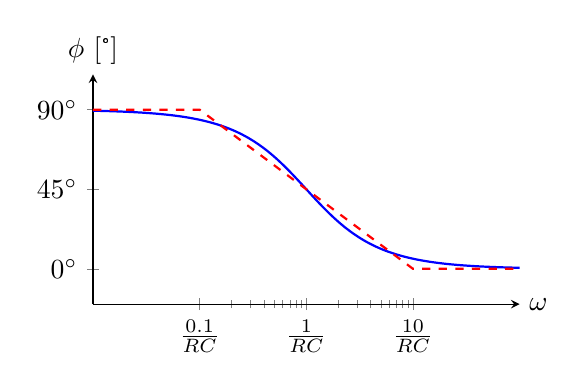
\begin{tikzpicture}
\begin{axis}[
    width=7cm, height=4.5cm,
    xmode=log,
    xlabel={$\omega$},
    ylabel={$\phi$ [°]},
    axis lines=left,
    xmin=0.1, xmax=100,
    xmin=0.01, xmax=100,
    ymin=-20, ymax=110,
    xtick={0.1, 1, 10}, xticklabels={$\frac{0.1}{RC}$, $\frac{1}{RC}$, $\frac{10}{RC}$},
    ytick={0, 45, 90}, yticklabels={$0^\circ$, $45^\circ$, $90^\circ$},
    domain=0.01:100, samples=200,
    every axis x label/.style={at={(ticklabel* cs:1)},anchor=west},
    every axis y label/.style={at={(ticklabel* cs:1)},anchor=south},
]
\addplot[blue, thick] {90 - atan(x)};
\addplot[red, dashed, thick] coordinates {(0.01,90) (0.1,90) (1,45) (10,0) (100,0)};
\end{axis}
\end{tikzpicture}
\end{fitcenter}

\subsubsection*{Filtro passa-banda}
\[
    \tilde{A}(s) = K \frac{s R_1 C_1}{(1+s R_1 C_1)(1+s R_2 C_2)}
\]

Supponendo $\frac{1}{R_1 C_1} \ll \frac{1}{R_2 C_2}$: la banda passante è compresa tra le due frequenze di taglio e in banda il modulo vale $|K|$ (nei grafici $K=1$, cioè $0$ dB). A sinistra di $\frac{1}{R_1 C_1}$ il diagramma cresce con $+20$ dB/decade (effetto dello zero in $s=0$); a destra di $\frac{1}{R_2 C_2}$ cala con $-20$ dB/decade. La fase parte da $+90^\circ$ (zero nell'origine), è circa $0^\circ$ in banda e tende a $-90^\circ$ ad alta frequenza.

\begin{fitcenter}
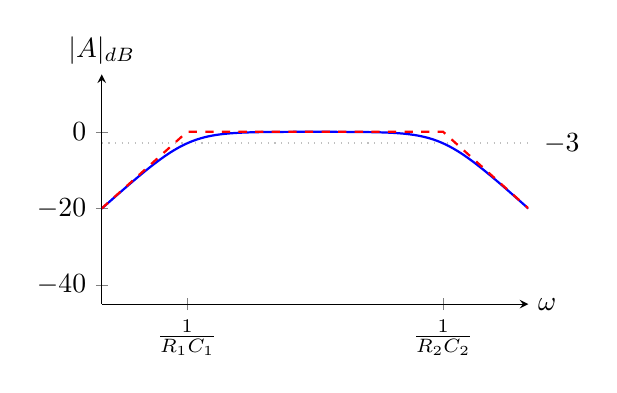
\begin{tikzpicture}
\begin{axis}[
    width=7cm, height=4.5cm,
    xmode=log,
    xlabel={$\omega$},
    ylabel={$|A|_{\text{dB}}$},
    axis lines=left,
    xmin=0.01, xmax=1000,
    ymin=-45, ymax=15,
    xtick={0.1, 100}, xticklabels={$\frac{1}{R_1 C_1}$, $\frac{1}{R_2 C_2}$},
    ytick={0,-20,-40},
    extra y tick style={grid=major, grid style={dotted,thick}, yticklabel pos=right},
    extra y ticks={-3},
    domain=0.01:1000, samples=200,
    every axis x label/.style={at={(ticklabel* cs:1)},anchor=west},
    every axis y label/.style={at={(ticklabel* cs:1)},anchor=south},
]
\addplot[blue, thick] {20*log10( (x*10) / sqrt((1+(x*10)^2)*(1+(x/100)^2)) )};
\addplot[red, dashed, thick] coordinates {(0.01,-20) (0.1,0) (100,0) (1000,-20)};
\end{axis}
\end{tikzpicture}
%
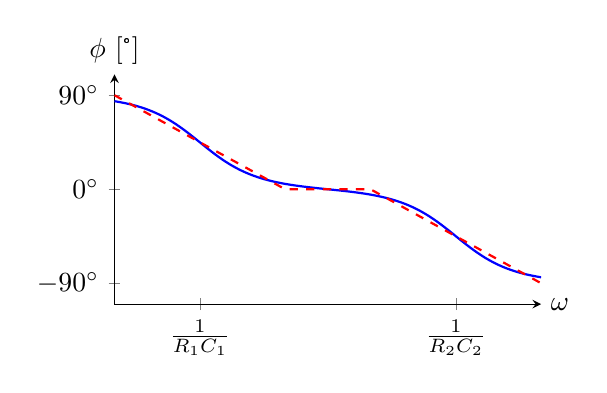
\begin{tikzpicture}
\begin{axis}[
    width=7cm, height=4.5cm,
    xmode=log,
    xlabel={$\omega$},
    ylabel={$\phi$ [°]},
    axis lines=left,
    xmin=0.01, xmax=1000,
    ymin=-110, ymax=110,
    xtick={0.1, 100}, xticklabels={$\frac{1}{R_1 C_1}$, $\frac{1}{R_2 C_2}$},
    ytick={-90, 0, 90}, yticklabels={$-90^\circ$, $0^\circ$, $90^\circ$},
    domain=0.01:1000, samples=200,
    every axis x label/.style={at={(ticklabel* cs:1)},anchor=west},
    every axis y label/.style={at={(ticklabel* cs:1)},anchor=south},
]
\addplot[blue, thick] {90 - atan(x*10) - atan(x/100)};
\addplot[red, dashed, thick] coordinates {(0.01,90) (1,0) (10,0) (1000,-90)};
\end{axis}
\end{tikzpicture}
\end{fitcenter}

\section*{Riepilogo del Capitolo e Trasformata di Laplace}

La \textbf{Trasformata di Laplace} è uno strumento matematico fondamentale per l'analisi dei circuiti, poiché converte equazioni differenziali nel dominio del tempo $t$ in equazioni algebriche nel dominio della variabile complessa $s$.

\begin{definizione}{Definizione e Convergenza}
La trasformata di Laplace di una funzione $f(t)$ è definita come:
\[
    \tilde{f}(s) = \mathcal{L}\{f(t)\} = \int_0^{+\infty} f(t)\, e^{-st} \, dt
\]
con $s \in \mathbb{C}$ appartenente al semipiano di convergenza.
Se esiste $s_0 = \sigma_0 + j\omega_0$ tale per cui l'integrale converge (ossia $|\tilde{f}(s_0)| \le \int_0^\infty \exp(-\sigma_0 t) |f(t)| dt < \infty$), allora la trasformata converge per ogni $s$ con $\text{Re}(s) \ge \sigma_0$.

\begin{note}La Trasformata di Fourier è una restrizione della Trasformata di Laplace alla sola retta immaginaria ($s = j\omega$) del piano complesso.\end{note}
\end{definizione}

\subsection*{Proprietà fondamentali}
\begin{itemize}
    \item \textbf{Linearità:} $\mathcal{L}\{\alpha_1 f_1(t) + \alpha_2 f_2(t)\} = \alpha_1 \mathcal{L}\{f_1(t)\} + \alpha_2 \mathcal{L}\{f_2(t)\}$
    \item \textbf{Convergenza:} Se $\tilde{f}(s_0)$ converge, allora $\tilde{f}(s)$ converge $\forall s \mid \text{Re}(s) \ge \sigma_0$.
    \item \textbf{Analiticità:} $\frac{d^n \mathcal{L}\{f\}}{ds^n} = (-1)^n \int_0^\infty t^n e^{-st} f(t) dt = (-1)^n \mathcal{L}\{t^n f(t)\}$ (se non presenta singolarità nel semipiano di convergenza).
    \item \textbf{Traslabilità:} $\mathcal{L}\{f(t) e^{at}\} = \tilde{f}(s-a)$
    \item \textbf{Convoluzione:} $\mathcal{L}\{(f * g)(t)\} = \tilde{f}(s) \cdot \tilde{g}(s)$, con $(f * g)(t) = \int_0^t f(\tau)g(t-\tau)\,d\tau$ (per funzioni causali)
\end{itemize}

\subsection*{Trasformate Notevoli}
\begin{center}
\renewcommand{\arraystretch}{1.5}
\begin{tabular}{ll | ll}
\toprule
\textbf{Funzione $f(t)$} & \textbf{Trasformata $\tilde{f}(s)$} & \textbf{Funzione $f(t)$} & \textbf{Trasformata $\tilde{f}(s)$} \\
\midrule
Impulso $\delta(t)$ & $1$ & Esponenziale $e^{at}$ & $\frac{1}{s-a}$ \\
Gradino $1$ & $\frac{1}{s}$ & Coseno $\cos(\omega t)$ & $\frac{s}{s^2+\omega^2}$ \\
Rampa $t$ & $\frac{1}{s^2}$ & Seno $\sin(\omega t)$ & $\frac{\omega}{s^2+\omega^2}$ \\
Potenza $t^n$ & $\frac{n!}{s^{n+1}}$ & Derivata $F'(t)$ & $s\tilde{F}(s) - F(0^+)$ \\
\bottomrule
\end{tabular}
\end{center}

\subsection*{Impedenze e Funzioni di Trasferimento}
Nel dominio di Laplace, i componenti reattivi diventano impedenze dipendenti da $s$:
\[
    Z_C(s) = \frac{1}{sC} \qquad \qquad Z_L(s) = sL
\]
Ad esempio, nel circuito $RC$ \textbf{integratore (filtro passa-basso)}, con $V_0$ tensione d'ingresso e $V_F$ tensione sul condensatore (condizioni iniziali nulle):
\[
    V_0 = RC \dot{V}_F + V_F \quad \xrightarrow{\text{Laplace}} \quad \tilde{V}_0(s) = sRC \tilde{V}_F(s) + \tilde{V}_F(s)
\]
Da cui si ricavano le funzioni di trasferimento:
\begin{itemize}
    \item \textbf{Filtro passa-basso}: $A_{LP}(s) = \frac{1}{1+sRC} = \left[ 1 + sRC \right]^{-1}$
    \item \textbf{Filtro passa-alto}: $A_{HP}(s) = \frac{sRC}{1+sRC} = \left[ 1 + (sRC)^{-1} \right]^{-1}$
\end{itemize}

\begin{note}
\textbf{Regole pratiche per i diagrammi di Bode asintotici:}
\begin{itemize}
    \item Ogni \textbf{polo reale negativo} $p_k$ introduce, alla frequenza $\omega = |p_k|$:
        \begin{itemize}
            \item variazione di pendenza di $-20$ dB/decade in ampiezza
            \item variazione di fase di $-90^\circ$
        \end{itemize}
    \item Ogni \textbf{zero reale negativo} $z_k$ introduce, alla frequenza $\omega = |z_k|$:
        \begin{itemize}
            \item variazione di pendenza di $+20$ dB/decade in ampiezza
            \item variazione di fase di $+90^\circ$
        \end{itemize}
    \item La frequenza alla quale il modulo vale $-3$ dB rispetto al valore di banda si chiama \textbf{frequenza di taglio}.
    \item Per un polo o uno zero reale semplice, il diagramma reale si discosta dall'asintotico di al massimo $3$ dB, proprio alla frequenza di rottura (per ordine $n$ lo scostamento è $3n$ dB). La fase asintotica si approssima con una retta che va da una decade prima a una decade dopo la frequenza di rottura.
\end{itemize}
\end{note}

\clearpage

